\subsection{Training}
The training is done by splitting the dataset into 70\% for train set, 15\% validation and 15\% test. The training execution was GPU-based on Google Colab.

A first training was done on the smaller data set consisting of 2000 images, to get a first look on the perfomances and change the model parameters to achieve the best performances with the model used. After this preliminary tunings it was used the full dataset of 50000 samples. The loss for each epoch is showed in figure \ref{fig:ValLoss}.


\begin{figure}[h!]
	\centering
	\begin{subfigure}{.5\textwidth}
		\centering
		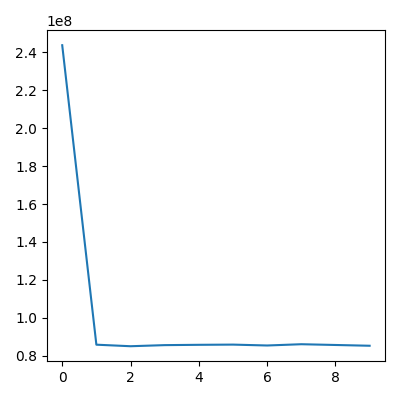
\includegraphics[width=0.4\linewidth]{./ImageFiles/Training/train-cost}
		\caption{Training loss vs epochs}
		\label{fig:TrainLoss}
	\end{subfigure}%
	\begin{subfigure}{.5\textwidth}
		\centering
		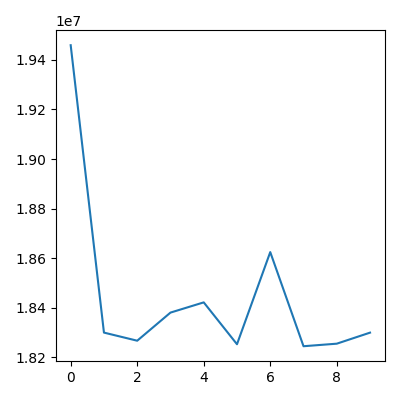
\includegraphics[width=0.4\linewidth]{./ImageFiles/Training/val-cost}
		\caption{Validation loss vs epochs}
		\label{fig:ValLoss}
	\end{subfigure}
	\caption{Loss vs epochs}
	\label{fig:ValLoss}
\end{figure}

The validation loss was used to tune the hyperparameters, that are learning rate, number of epochs and batch size. The best emerged values are learning rate 0.001, 10 epochs and batch size 500.